
\textbf{Definition Stetigkeit:}\\
$\forall \epsilon > 0 :\exists \delta > 0 : |x-a|<\delta : |f(x)-f(a)|<\epsilon$\\
$\forall \epsilon > 0 :\exists \delta > 0 : f(U_{\delta}(a) \subseteq U_{\epsilon}(f(a)))$\\
$\forall \epsilon > 0\  \exists \delta >0 : \text{sodass aus } |x-a|<\delta \text{ stets } |f(x)-f(a)|<\epsilon \text{ folgt}$\\

\textbf{Definition Unstetigkeit:} $\exists \epsilon > 0 \forall\  \delta > 0 :\exists x \in D : |x-x_0|< \delta \wedge |f(x)-f(x_0)|>\epsilon$

\subsection{links-rechtsseitiger Grenzwetz:}

$\lim\limits_{x\to x_0^-}f(x) = \lim\limits_{x\to x_0^+} f(x)$

$x_0$ wird von rechts und links angenähert. Sind beide Grenzwerte gleich, ist die Funktion stetig.


\subsection{\(\epsilon - \delta\) Kriterium}



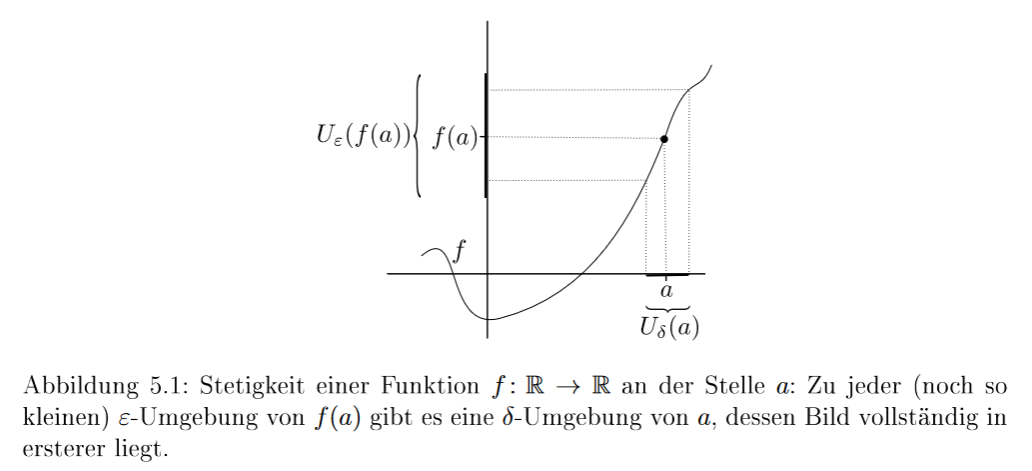
\includegraphics[width= \textwidth]{./pictures/Stetigkeit.png}

\textbf{Stetigkeit zeigen:}
\begin{itemize}
    \item $|f(x)-f(a)|<\epsilon$ aufstellen
    \item alle $x$ rausbringen ($x-a = \delta$, manchmal einfügen einer geschickten Null ($+ a - a$))
    \item Formel auf $\delta=$ umformen
    \item das berechnete $\delta$ in dne Beweis einsetzen
    \item Wahre Aussage
\end{itemize}



